\documentclass{beamer}[10]

\usepackage{graphicx}
\usepackage{xcolor}
\usepackage{tabto}
%\usepackage{beamerthemesplit}
\usepackage{tikz}
\usepackage{cancel}
\usepackage{verbatim}
\usepackage{fancybox}
\usepackage{enumerate}
\usepackage{amsmath,amssymb,amsthm,textcomp,mathtools}
\usepackage[super]{nth}
\usepackage[amssymb]{SIunits}
\usepackage{booktabs}
\usepackage{cancel}
\usepackage{bm}
\usepackage[utf8]{inputenc}
\usepackage{tabularx}
\usepackage{ragged2e}
\newcolumntype{Y}{ >{\RaggedRight\arraybackslash}X}
\usetikzlibrary{arrows,shapes}
\newcommand\T{\rule{0pt}{2.6ex}}
\newcommand\B{\rule[-1.2ex]{0pt}{0pt}}
\definecolor{UUcrimson}{RGB}{204,0,0}
\mode<presentation>
{ \usetheme{default}
  \usecolortheme[named=UUcrimson]{structure}
  \useinnertheme{circles}
  \setbeamercovered{transparent}
  \setbeamertemplate{blocks}[rounded]
  \usefonttheme[onlymath]{serif}
  \setbeamertemplate{navigation symbols}{}
  \setbeamertemplate{footline}[page number]
  \setbeamertemplate{navigation symbols}{}
  \setbeamercolor{section in toc}{fg=black,bg=white}
  \setbeamercolor{alerted text}{fg=UUcrimson!80!gray}
  \setbeamercolor*{palette primary}{fg=white,bg=UUcrimson}
  \setbeamercolor*{palette secondary}{fg=UUcrimson!70!black,bg=gray!15!white}
  \setbeamercolor*{palette tertiary}{bg=UUcrimson!80!black,fg=gray!10!white}
  \setbeamercolor*{palette quaternary}{fg=UUcrimson,bg=gray!5!white}
  \setbeamercolor*{palette sidebar primary}{fg=UUcrimson!10!black}
  \setbeamercolor*{palette sidebar secondary}{fg=white}
  \setbeamercolor*{palette sidebar tertiary}{fg=UUcrimson!50!black}
  \setbeamercolor*{palette sidebar quaternary}{fg=gray!10!white}
  \setbeamercolor{titlelike}{parent=palette primary,fg=white}
  \setbeamercolor{frametitle}{bg=UUcrimson}
  \setbeamercolor{frametitle right}{bg=UUcrimson}
  \setbeamercolor*{separation line}{}
  \setbeamercolor*{fine separation line}{}
}

\usetikzlibrary{backgrounds}
\makeatletter
\tikzstyle{every picture}+=[remember picture]
\tikzset{%
  fancy quotes/.style={
    text width=\fq@width pt,
    align=justify,
    inner sep=1em,
    anchor=north west,
    minimum width=\linewidth,
    font=\itshape
  },
  fancy quotes width/.initial={.8\linewidth},
  fancy quotes marks/.style={
    scale=8,
    text=white,
    inner sep=0pt,
  },
  fancy quotes opening/.style={
    fancy quotes marks,
  },
  fancy quotes closing/.style={
    fancy quotes marks,
  },
  fancy quotes background/.style={
    show background rectangle,
    inner frame xsep=0pt,
    background rectangle/.style={
      fill=gray!25,
      rounded corners,
    },
  }
}
\newenvironment{fancyquotes}[1][]{%
\noindent
\tikzpicture[fancy quotes background]
\node[fancy quotes opening,anchor=north west] (fq@ul) at (0,0) {``};
\tikz@scan@one@point\pgfutil@firstofone(fq@ul.east)
\pgfmathsetmacro{\fq@width}{\linewidth - 2*\pgf@x}
\node[fancy quotes,#1] (fq@txt) at (fq@ul.north west) \bgroup}
{\egroup;
\node[overlay,fancy quotes closing,anchor=east] at (fq@txt.south east) {''};
\endtikzpicture}
\makeatother


\usetikzlibrary{backgrounds}
\makeatletter
\tikzstyle{every picture}+=[remember picture]
\tikzset{%
  fancy defs/.style={
    text width=\fq@width pt,
    align=justify,
    inner sep=0.25em,
    anchor=north west,
    minimum width=\linewidth,
    font=\itshape
  },
  fancy defs width/.initial={.8\linewidth},
  fancy defs marks/.style={
    scale=8,
    text=white,
    inner sep=0pt,
  },
  fancy defs opening/.style={
    fancy defs marks,
  },
  fancy defs closing/.style={
    fancy defs marks,
  },
  fancy defs background/.style={
    show background rectangle,
    inner frame xsep=0pt,
    background rectangle/.style={
      fill=gray!25,
      rounded corners,
    },
  }
}
\newenvironment{fancydefs}[1][]{%
\noindent
\tikzpicture[fancy defs background]
\node[fancy defs opening,anchor=north west] (fq@ul) at (0,0) {};
\tikz@scan@one@point\pgfutil@firstofone(fq@ul.east)
\pgfmathsetmacro{\fq@width}{\linewidth - 2*\pgf@x}
\node[fancy defs,#1] (fq@txt) at (fq@ul.north west) \bgroup}
{\egroup;
\node[overlay,fancy defs closing,anchor=east] at (fq@txt.south east) {};
\endtikzpicture}
\makeatother
\usepackage{scalerel}[2014/03/10]
\usepackage{stackengine}
\usepackage{empheq}
\newcommand*\widefbox[1]{\fbox{\hspace{0.5em}#1\hspace{0.5em}}}

\newcommand\reallywidetilde[1]{\ThisStyle{%
  \setbox0=\hbox{$\SavedStyle#1$}%
  \stackengine{-.1\LMpt}{$\SavedStyle#1$}{%
    \stretchto{\scaleto{\SavedStyle\mkern.2mu\sim}{.5467\wd0}}{.4\ht0}%
%    .2mu is the kern imbalance when clipping white space
%    .5467++++ is \ht/[kerned \wd] aspect ratio for \sim glyph
  }{O}{c}{F}{T}{S}%
}}
\usepackage{media9}

\logo{
\includegraphics[width=0.75cm]{logo.jpg}}
\author[Gibbs]{Dr. Jeremy A. Gibbs}
\institute{Department of Mechanical Engineering\\University of Utah}
\date{Spring 2017}
\title{Environmental Fluid Dynamics: Lecture 19}
% colors
\usepackage[loadonly]{enumitem}
\newcommand{\ihat}{\boldsymbol{\hat{\imath}}}
\newcommand{\jhat}{\boldsymbol{\hat{\jmath}}}
\newcommand{\khat}{\boldsymbol{\hat{k}}}
\definecolor{colororange}{HTML}{E65100} % orange
\definecolor{colordgray}{HTML}{795548} % dark gray for note
\definecolor{colorhgray}{HTML}{212121} % heavy dark gray for normal text
\definecolor{colorgreen}{HTML}{009688} % green
\definecolor{colorwhite}{HTML}{FFFFFF} % background white
\definecolor{colorlgray}{HTML}{F5F3EE} % background light gray
\definecolor{colorblue}{HTML}{0277BB} % blue
\definecolor{colorred}{HTML}{CC0000} % red
\newcommand{\fontsizeone}{1.9em}
\usepackage{esvect}
\setbeamertemplate{caption}{\raggedright\insertcaption\par}
\newcommand{\framecard}[2][colorgreen]{
  {\setbeamercolor{background canvas}{bg=#1}
    \begin{frame}[plain]
    \vfill
    \begin{center}
     {#2}
    \end{center}
    \vfill
    \end{frame}
  }
}
\begin{document}

%----------------------------------------------------------------------------------------
%	TITLE & TOC SLIDES
%----------------------------------------------------------------------------------------

\begin{frame} 
  \titlepage
\end{frame}

%------------------------------------------------

\begin{frame}
\frametitle{Overview}
\tableofcontents
\end{frame}

%------------------------------------------------
\section{Dynamic Instability in the Atmosphere} %
%------------------------------------------------
\subsection{Stability Overview}
%------------------------------------------------
\framecard[colorred]{{\color{white}\Huge Stability Review}}
%------------------------------------------------
\begin{frame}{Stability Review}
\begin{itemize}
	\item In the broadest sense, stability is a dividing line between laminar and turbulent flows.
	\item If a flow is stable, it can become or remain laminar.
	\item If a flow is unstable, it can become or remain turbulent.
	\item There are many stabilizing and destabilizing factors to consider.
\end{itemize}
\end{frame}
%------------------------------------------------
\begin{frame}{Stability Review}

\begin{itemize}
	\item These factors are often terms in the TKE balance equation
	\item To simplify and understand the problem, a destabilizing term is often paired with a stabilizing term to form a dimensionless ratio.
	\item This ratio is used to determine which factor "wins" and whether the flow becomes turbulent or not.
	\item Examples include the Reynolds number, Richardson number, Rossby number, Rayleigh number, and Froude number.
\end{itemize}
\end{frame}
%------------------------------------------------
\begin{frame}{Stability Review}
\begin{itemize}
	\item Recall that we previously discussed static stability.
	\item ``Static'' means no motion, so it described stability that is independent of the wind.
	\item Static stability determined whether a flow was capable of buoyant convection.
	\item Hence, we framed our discussion of static stability around vertical profiles of potential temperature.
	\item  Today we will discuss dynamic instability.  
\end{itemize}
\end{frame}
%------------------------------------------------
\subsection{Dynamic Instability}
%------------------------------------------------
\framecard[colorred]{{\color{white}\Huge Dynamic Instability}}
%------------------------------------------------
\begin{frame}{Dynamic Instability}
\begin{itemize}
	\item ``Dynamic'' means having motion
	\item Unlike static stability, dynamic stability depends on the wind
	\item Even if the atmosphere is statically stable in some layer, wind shear may be sufficient to generate turbulence
	\item One example is Kelvin-Helmholtz instability
\end{itemize}
\end{frame}
%------------------------------------------------
\begin{frame}{Dynamic Instability: Kelvin-Helmholtz}
\begin{columns}[T]
    \begin{column}{.3\textwidth}
    	\begin{minipage}[c][0.75\textheight][c]{\linewidth}
    		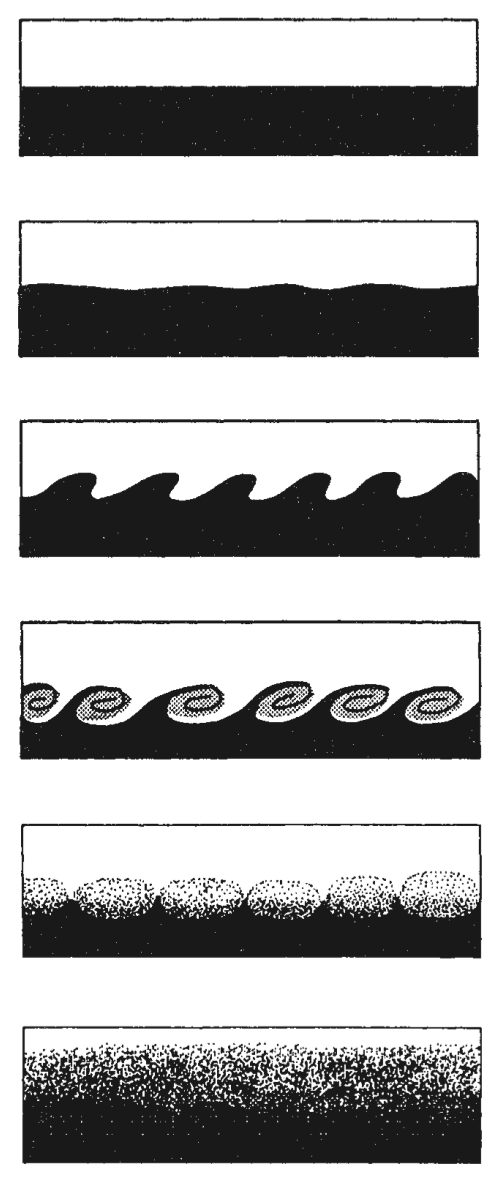
\includegraphics[width=\textwidth]{kh}
    	\end{minipage}
    \end{column}
    \begin{column}{.7\textwidth}
    	\begin{itemize}
    		\item Consider low density fluid on top of high density fluid (statically stable)
    		\item Imagine that shear ($\Delta U$) exists at their interface.
    		\item If shear becomes large enough, the flow is dynamically unstable,
    		\item The amplitude of the waves grows until they break.
    		\item The breaking wave is called a Klevin-Helmholtz (KH) wave.
    		\item The physics are different than a breaking wave on the ocean's surface, for instance.
    	\end{itemize}
    \end{column}
  \end{columns}
\end{frame}
%------------------------------------------------
\begin{frame}{Dynamic Instability: Kelvin-Helmholtz}
\begin{columns}[T]
    \begin{column}{.3\textwidth}
    	\begin{minipage}[c][0.75\textheight][c]{\linewidth}
    		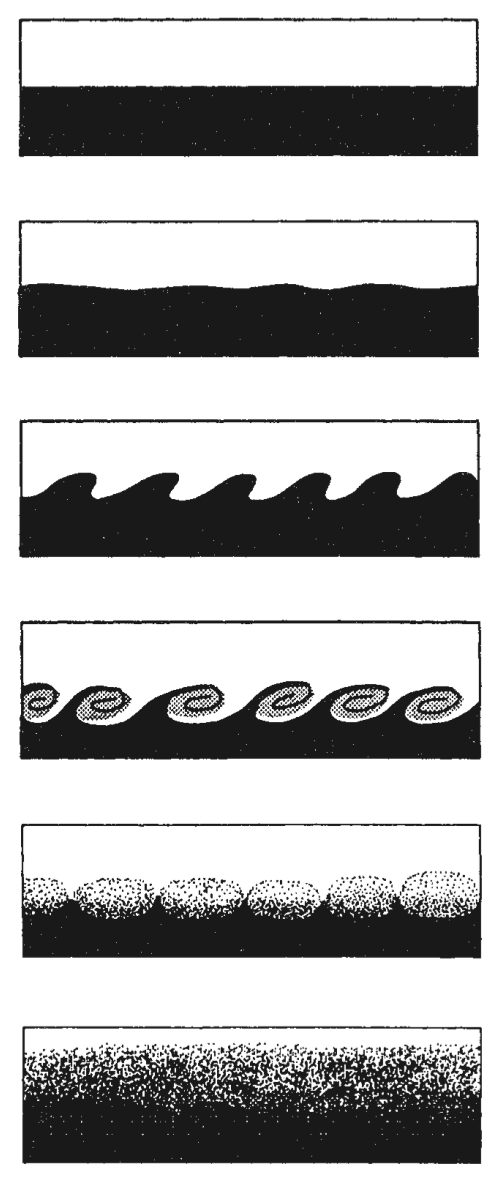
\includegraphics[width=\textwidth]{kh}
    	\end{minipage}
    \end{column}
    \begin{column}{.7\textwidth}
    	\begin{itemize}
    		\item Within each wave roll there are ``packets'' of statically unstable fluid (locally heavy above light fluid)
    		\item The static and dynamic instabilities act to generate turbulence.
    		\item The turbulence expands and leads to diffusion (mixing), which transfers momentum and reduces the shear.
    		\item If the shear falls below the critical value, then the dynamic instability ends.
    		\item In the absence of the shear, turbulence decays and the flow becomes laminar.
    	\end{itemize}
    \end{column}
  \end{columns}
\end{frame}
%------------------------------------------------
\begin{frame}{Dynamic Instability: Kelvin-Helmholtz}
\begin{itemize}
	\item KH waves likely occur often in statically-stable shear layers, although they are rarely observed visually.
	\item If sufficient moisture is present in the atmosphere, clouds can form in the ascending portions of the wave.
	\item These are called billow clouds.
\end{itemize}
\end{frame}
%------------------------------------------------
\begin{frame}{Dynamic Instability: Kelvin-Helmholtz}
\begin{figure}
	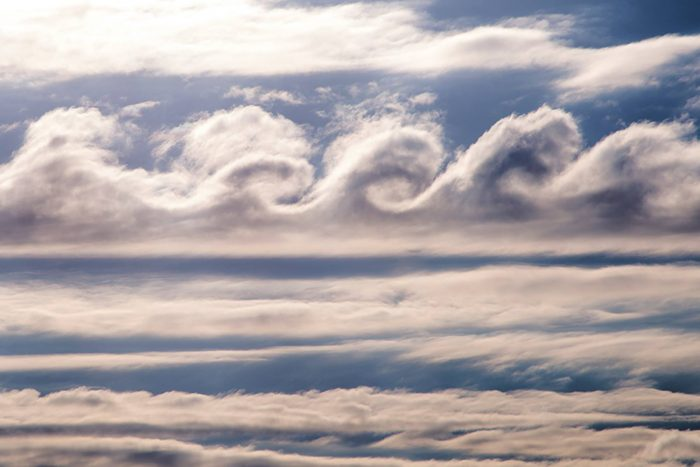
\includegraphics[width=\textwidth]{kh2}
\end{figure}
\small{photo by Paul Chartier, via: Earthsky.org}
\end{frame}
%------------------------------------------------
\begin{frame}{Dynamic Instability}
\begin{itemize}
	\item Interestingly, both static and dynamic instabilities cause the flow to react in a way to remove the instability.
	\item So, turbulence is an "effort" by the flow to undo the cause of the instability.
	\item Static: convection moves buoyant air upward, which stabilizes the flow.
	\item Dynamic: turbulence reduces wind shears, which stabilizes the flow.
\end{itemize}
\end{frame}
%------------------------------------------------
\begin{frame}{Dynamic Instability}
\begin{itemize}
	\item In other words, turbulence exists to end its own existance
	\begin{figure}
		
\includegraphics[width=0.7\textwidth]{mindblown}
	\end{figure}
\end{itemize}
\end{frame}
%------------------------------------------------
\begin{frame}{Dynamic Instability}
\begin{itemize}
	\item Since observations show prolonged periods of turbulence in the atmosphere, there must be external forces that act to destabilize the PBL.
	\item Static: solar heating of ground.
	\item Dynamic: pressure gradients from synoptic-scale features causes winds to fight dissipation.
\end{itemize}
\end{frame}
%------------------------------------------------
\begin{frame}{Dynamic Instability}
\begin{itemize}
	\item To understand when a flow might become dynamically unstable, we can compare the relative magnitudes of the shear and buoyancy terms in our TKE balance equation.
	\item Shear leads to mechanical production of turbulence - a destabilizing effect.
	\item Buoyancy can either enhance or suppress turbulence - so it can be stabilizing or destabilizing.
	\item One such ratio is the Richardson number Ri.
\end{itemize}
\end{frame}
%------------------------------------------------
\subsection{Richardson Number}
%------------------------------------------------
\framecard[colorred]{{\color{white}\Huge Richardson Number}}
%------------------------------------------------

\begin{frame}{Dynamic Instability: Flux Richardson Number}
\begin{itemize}
	\item Consider a statically-stable environment.
	\item turbulent motions have to fight gravity, so buoyancy suppresses turbulence here.
	\item Conversely, wind shear acts to generate turbulence.
	\item The buoyant production/consumption term in the TKE balance is negative and the shear production term is positive.
	\item It is useful to examine their ratio.
\end{itemize}
\end{frame}
%------------------------------------------------
\begin{frame}{Dynamic Instability: Flux Richardson Number}
\begin{itemize}
	\item The ratio of buoyant production/consumption to shear production is called the \textbf{Flux Richardson Number}:
	$$\mathrm{Ri_f} = \frac{ \left(\cfrac{g}{\overline{\theta_v}}\right) (\overline{w^\prime \theta_v^\prime})}{(\overline{u_i^\prime u_j^\prime})\cfrac{\partial \overline{u_i}}{\partial x_j}} = \frac{(\overline{w^\prime b^\prime})}{(\overline{u_i^\prime u_j^\prime})\cfrac{\partial \overline{u_i}}{\partial x_j}}$$
	\item The Richardson number is dimensionless and contains nine terms int he denominator!
\end{itemize}
\end{frame}
%------------------------------------------------
\begin{frame}{Dynamic Instability: Flux Richardson Number}
\begin{itemize}
	\item If we neglect subsidence ($\overline{w}=0$) and assume horizontal homogeneity, we arrive:
	$$\mathrm{Ri_f} = \frac{ \left(\cfrac{g}{\overline{\theta_v}}\right) (\overline{w^\prime \theta_v^\prime})}{(\overline{u^\prime w^\prime})\cfrac{\partial \overline{u}}{\partial z} + (\overline{v^\prime w^\prime})\cfrac{\partial \overline{v}}{\partial z}} = \frac{(\overline{w^\prime b^\prime})}{(\overline{u^\prime w^\prime})\cfrac{\partial \overline{u}}{\partial z} + (\overline{v^\prime w^\prime})\cfrac{\partial \overline{v}}{\partial z}}$$
\end{itemize}
\end{frame}
%------------------------------------------------
\begin{frame}{Dynamic Instability: Flux Richardson Number}
\begin{itemize}
	\item For statically stable, unstable, neutral flows, $\mathrm{Ri_f}$ is positive, negative, 0 - respectively.
	\item Richardson suggested $\mathrm{Ri_f}=1$ is a critical value since mechanical and buoyant terms are in balance.
	\item At any value less than $\mathrm{Ri_f}=1$, static stability is too weak to prevent mechanical generation of turbulence.
	\item For $\mathrm{Ri_f}<1$, buoyancy contributes to the generation of turbulence.
	\begin{gather*}
	\begin{cases}
	\text{Flow is dynamically unstable (turbulent)} & \mathrm{Ri_f}<1\\
	\text{Flow is dynamically stable (laminar)} & \mathrm{Ri_f}>1
	\end{cases}
	\end{gather*}
	\item Note: statically unstable flow is by definition dynamically unstable.
\end{itemize}
\end{frame}
%------------------------------------------------
\begin{frame}{Dynamic Instability: Gradient Richardson Number}
\begin{itemize}
	\item With $\mathrm{Ri_f}$, notice that our terms involve turbulent fluxes.
	\item So, it determines when a turbulent flow becomes laminar, but not when a laminar flow becomes turbulent.
	\item Using the idea of $K$-theory, we can say that $-\overline{w^\prime \theta_v^\prime}$ is proportional to $\partial \overline{\theta_v}/\partial z$,$-\overline{u^\prime w^\prime}$ is proportional to $\partial \overline{u}/\partial z$, and $-\overline{v^\prime w^\prime}$ is proportional to $\partial \overline{v}/\partial z$.
	\item We can use these assumptions to create a new Richardson number.
\end{itemize}
\end{frame}
%------------------------------------------------
\begin{frame}{Dynamic Instability: Gradient Richardson Number}
\begin{itemize}
	\item The \textbf{Gradient Richardson Number} is given by:
	$$\mathrm{Ri} = \frac{\cfrac{g}{\overline{\theta_v}} \left(\cfrac{\partial \overline{\theta_v}}{\partial z}\right)}{\left(\cfrac{\partial \overline{u}}{\partial z}\right)^2 + \left(\cfrac{\partial \overline{v}}{\partial z}\right)^2}$$
	\item If you see $\mathrm{Ri}$ without any subscript - the authors probably mean the gradient Richardson number.
\end{itemize}
\end{frame}
%------------------------------------------------
\begin{frame}{Dynamic Instability: Gradient Richardson Number}
\begin{itemize}
	\item Theoretical and experimental data suggest that laminar flow becomes turbulent when $\mathrm{Ri}$ is below a critical value $\mathrm{Ri_c}$, while turbulent flow ceases at some termination value $\mathrm{Ri_t}$.
	\begin{gather*}
	\begin{cases}
	\text{Laminar flow becomes turbulent} & \mathrm{Ri}<\mathrm{Ri_c}\\
	\text{Turbulent flow becomes laminar} & \mathrm{Ri}>\mathrm{Ri_t}
	\end{cases}
	\end{gather*}
	\item There is still debate about what values should be used, but typically $\mathrm{Ri_c} = 0.25$ and $\mathrm{Ri_t} = 1$.
	\item There is a hysteresis since $\mathrm{Ri_t} > \mathrm{Ri_c}$
\end{itemize}
\end{frame}
%------------------------------------------------
\begin{frame}{Dynamic Instability: Gradient Richardson Number}
\textbf{Why the hysteresis?}
\begin{itemize}
	\item The idea is that we need two conditions for turbulence: instability and a trigger mechanism.
	\item Consider KH waves as a trigger mechanism.
	\item In the absence of existing turbulence, $\mathrm{Ri}$ must fall well below $\mathrm{Ri_t}$ in order for KH waves to form.
	\item Experimental data suggests KH waves form when $\mathrm{Ri}<\mathrm{Ri_c}$.
\end{itemize}
\end{frame}
%------------------------------------------------
\begin{frame}{Dynamic Instability: Gradient Richardson Number}
\textbf{Why the hysteresis?}
\begin{itemize}
	\item Thus, we have a hysteresis.
	\item In other words, the Richardson number of a non-turbulent flow must be lowered to $\mathrm{Ri_c}$, while a turbulent flow can remain so until the Richardson number surpasses $\mathrm{Ri_t}$.
\end{itemize}
\end{frame}
%------------------------------------------------
\begin{frame}{Dynamic Instability: Bulk Richardson Number}

\begin{itemize}
	\item $\mathrm{Ri_c}\approxeq 0.25$ is theoretically based on local gradients of wind and temperature.
	\item In the real world, we don't really know those local gradients.
	\item However, we can approximate them using discrete height layers.
	\item For example, we can approximate $\partial \overline{\theta_v}/\partial z$ as $\Delta \overline{\theta_v} / \Delta z$.
	\item We can apply these approximations to the gradient Richardson number to create a new ratio.
\end{itemize}
\end{frame}
%------------------------------------------------
\begin{frame}{Dynamic Instability: Bulk Richardson Number}

\begin{itemize}
	\item The \textbf{Bulk Richardson Number} is given by:
	\begin{align*}
	\mathrm{Ri_B} &= \frac{ \cfrac{g}{\overline{\theta_v}} \cfrac{\Delta \overline{\theta_v}}{\Delta z}}{\left(\cfrac{\Delta \overline u}{\Delta z}\right)^2 + \left(\cfrac{\Delta \overline v}{\Delta z}\right)^2} = \frac{g \Delta \overline{\theta_v} \Delta z}{\overline{\theta_v} \left[(\Delta \overline u)^2 + (\Delta \overline v)^2\right]}
	\end{align*}
	\item This is the form most often used by meteorologists.
	\item Observational and NWP data give wind and temperature at discrete points in the vertical.
	\item Note: $\Delta \overline{u} = \overline{u}(\text{top}) - \overline{u}(\text{bottom})$
\end{itemize}
\end{frame}
%------------------------------------------------
\begin{frame}{Dynamic Instability: Bulk Richardson Number}

\begin{itemize}
	\item A few words of caution with $\mathrm{Ri_B}$ are warranted.
	\item The critical value is based on local gradients and not finite differences across layers.
	\item Gradients likely get ``washed out'' as the layer grows in thickness.
	\item Uncertainty arises in our ability to determine whether turbulence might form.
	\item Since some observations are spread far apart in the vertical, we must take care in interpreting the computed $\mathrm{Ri_B}$ when trying to characterize the considered flow.
\end{itemize}
\end{frame}
%------------------------------------------------

\end{document}

